\documentclass[conference]{IEEEtran}

\usepackage{amsmath,amssymb}
\usepackage{booktabs}
\usepackage{graphicx}
\usepackage{multirow}
\usepackage{url}
\usepackage{xcolor}
\usepackage{balance}
\graphicspath{{../artifacts/}}

\title{SecGuard: ML-Driven Risk-Adaptive Isolation for\\
Profit-Aware End-to-End 5G Network Slicing}

\author{\IEEEauthorblockN{Anonymous Author(s)}
\IEEEauthorblockA{Master's Thesis Project\\
Institution and email to be added}}

\begin{document}
\maketitle

\begin{abstract}
End-to-end network slicing permits heterogeneous services to share radio,
transport, and compute infrastructure, but this sharing creates a tension between
security isolation and infrastructure efficiency. 5Guard addresses this tension
by embedding slice requests at one of three isolation levels; however, the
isolation level is supplied with the request and is not adapted to runtime attack
evidence. This paper presents SecGuard, a preliminary machine-learning-driven
extension that converts 5G packet and GTP telemetry into a per-slice attack-risk
score, applies an SLA-safe isolation action, and feeds the resulting request to
the original 5Guard allocator. A Random Forest classifier is trained on 30,288
records and evaluated on a separate 3,787-record test file. A second pair of
Random Forest regressors learns the relationship between isolation thresholds,
5Guard profit, and a transparent isolation-exposure proxy from Gurobi-backed
offline evaluations. The learned policy is chosen under a minimum predicted
security-improvement constraint. On 30 held-out trace-derived scenarios using
5Guard's IAR algorithm and synthetic topology, learned SecGuard improves mean
profit by 164.92\% and slice admission by 27.94\% relative to a fixed-threshold
SecGuard policy. Compared with static 5Guard, it retains 90.44\% of mean profit
while reducing modeled isolation exposure by 67.12\%. These results establish
feasibility and expose a useful security--profit trade-off; broader topologies,
cross-dataset testing, and measured attack propagation remain necessary before
deployment or generalization claims.
\end{abstract}

\begin{IEEEkeywords}
5G, network slicing, slice isolation, intrusion detection, machine learning,
resource allocation, security orchestration.
\end{IEEEkeywords}

\section{Introduction}
Network slicing creates multiple logical networks over a common 5G
infrastructure. This enables an infrastructure provider to serve heterogeneous
verticals, but co-residency permits failures or attacks in one slice to influence
other tenants. Standards therefore recognize differentiated security capabilities
and runtime monitoring of isolation \cite{itutx1816,itutx1814,3gppts33501}.
Applying complete physical isolation to every slice is nevertheless expensive:
dedicated radio, transport, and compute resources reduce multiplexing gains and
can lower admission and profit.

5Guard formalizes isolation-aware end-to-end slicing with three levels---L0,
L1, and L2---and accounts for resource overhead, migration, priority, and QoS
violations \cite{bolourian2026fiveguard}. It selects the best solution returned
by an ensemble of exact and approximate algorithms within the allocation
deadline. A remaining gap is that the requested isolation level is static. The
allocator does not consume runtime traffic evidence and cannot decide whether a
slice should retain, strengthen, or leave the shared substrate after its risk
changes.

This paper investigates the following question:

\begin{quote}
Can telemetry-derived risk dynamically control 5Guard isolation while recovering
the profit lost by a conservative security policy?
\end{quote}

SecGuard adds two learning stages around 5Guard. First, a supervised classifier
maps 5G packet/GTP features to attack probability and aggregates those
probabilities into a slice risk. Second, a profit-aware surrogate learns the
outcomes of 5Guard allocations under candidate L1, L2, and quarantine
thresholds. The selected thresholds maximize predicted profit subject to a
minimum exposure-reduction constraint. A safety floor guarantees that SecGuard
never assigns weaker isolation than the customer's SLA.

The contributions are:

\begin{itemize}
  \item an end-to-end telemetry--risk--isolation adapter for the original
  5Guard slice-request class, including explicit quarantine semantics;
  \item an SLA-safe dynamic isolation policy and a transparent risk-weighted
  isolation-exposure proxy;
  \item a constrained ML surrogate that learns profit-aware thresholds from
  actual Gurobi-backed 5Guard outcomes rather than an analytical cost shortcut;
  \item a reproducible preliminary evaluation with held-out scenarios, paired
  confidence intervals, source code, tests, and limitations.
\end{itemize}

\section{Background and Related Work}
\subsection{Isolation-aware slicing}
5Guard models radio units, network functions, and virtual paths mapped to NR base
stations, physical servers, and transport paths \cite{bolourian2026fiveguard}.
L0 permits sharing, L1 adds logical or semi-isolation overhead, and L2 reserves
physical entities. Its formulation captures deployment cost, overhead,
migration, and controlled QoS violations. The published system reports profit
and admission improvements over its individual algorithms, but its conclusion
identifies translating security requirements into isolation levels as future
work. SecGuard targets precisely that boundary and reuses the published data
model and allocator \cite{fiveguardcode}.

ITU-T X.1816 classifies differentiated network-slice security capabilities and
recognizes resource isolation as a selectable capability \cite{itutx1816}.
ITU-T X.1814 further calls for runtime monitoring and updating of slice isolation
when needed \cite{itutx1814}. These recommendations motivate a controller that
can strengthen isolation based on current risk without applying uniform L2.

\subsection{ML security and admission control}
Prior work uses reinforcement learning to mitigate DDoS effects through slice
isolation \cite{javadpour2023isolation} and deep reinforcement learning for joint
admission and embedding \cite{troia2022admission}. Explainability studies show
that learned admission controllers can become overly conservative, rejecting
feasible requests based mainly on substrate congestion \cite{asdikian2025verifying}.
Predictive admission has also been coupled to capacity forecasts under weather
uncertainty \cite{jacoby2026aware}. These studies demonstrate the value of
learning but do not provide SecGuard's combination of telemetry-derived security
risk, three-level end-to-end isolation, SLA flooring, quarantine, and
profit-constrained threshold selection over the 5Guard model.

\section{System Model and Problem Statement}
At decision epoch $t$, a slice $i$ has an SLA isolation requirement
$\gamma_i^{\mathrm{SLA}}\in\{0,1,2\}$, service class, resource graph, revenue,
and allocation deadline. A classifier observes a window of $n_i$ packet records
and outputs attack probabilities $p_{ij}$. SecGuard defines slice risk as
\begin{equation}
 r_i = \frac{1}{n_i}\sum_{j=1}^{n_i}p_{ij}.
 \label{eq:risk}
\end{equation}

Let thresholds $\boldsymbol{\tau}=(\tau_1,\tau_2,\tau_q)$ satisfy
$0\leq\tau_1<\tau_2<\tau_q\leq1$. The risk floor is
\begin{equation}
 \gamma_i^{\mathrm{risk}} =
 \begin{cases}
  0, & r_i < \tau_1,\\
  1, & \tau_1\leq r_i < \tau_2,\\
  2, & \tau_2\leq r_i < \tau_q.
 \end{cases}
\end{equation}
For non-quarantined requests, the optimizer receives
\begin{equation}
 \gamma_i = \max\left(\gamma_i^{\mathrm{SLA}},
                       \gamma_i^{\mathrm{risk}}\right).
 \label{eq:sla-floor}
\end{equation}
If $r_i\geq\tau_q$, the request is withheld from the shared allocator. Equation
\eqref{eq:sla-floor} is a hard safety invariant: learning cannot weaken the
contracted isolation.

\subsection{Isolation-exposure proxy}
The present simulator does not propagate attacks. We therefore define a clearly
labeled proxy rather than claiming measured containment. Let $w_i$ denote
service impact and $s(\gamma)$ a sharing factor with $s(0)=1$, $s(1)=0.5$, and
$s(2)=s(q)=0$. Exposure is
\begin{equation}
 E(\boldsymbol{\tau}) = \sum_i r_i w_i s(\gamma_i).
 \label{eq:exposure}
\end{equation}
The value 0.5 for L1 is an initial modeling assumption. It must be varied in a
sensitivity analysis and later replaced by placement-derived or testbed-measured
sharing.

Let $P(\boldsymbol{\tau})$ be the final raw profit returned by 5Guard. Threshold
learning seeks
\begin{align}
 \max_{\boldsymbol{\tau}}\quad & \widehat{P}(\boldsymbol{\tau}) \\
 \mathrm{s.t.}\quad & \widehat{E}(\boldsymbol{\tau})
 \leq (1-\eta)E_{\mathrm{static}},
 \label{eq:optimization}
\end{align}
where $\eta=0.60$ is the required predicted exposure reduction and the hats denote
learned surrogates.

\section{SecGuard Design}
\subsection{Telemetry risk model}
The first stage uses a Random Forest classifier \cite{breiman2001random}. It is
trained on two dataset-provided files containing 30,288 records and 44 IP, TCP,
UDP, frame, and GTP features. The official 3,787-record test file is held out.
Class-balanced bootstrap weights reduce bias toward benign traffic. The model
has 300 trees, depth 18, minimum leaf size two, and seed 42.

The data originate from an Open5GS/UERANSIM environment and contain normal
traffic and simulated DDoS, PFCP, and IP-spoofing anomalies
\cite{sheikhi2023ddos,open5gsdataset}. Packet scores are aggregated using
\eqref{eq:risk}. Mean aggregation is simple and interpretable, though future
work should compare maxima, quantiles, and temporal models.

\subsection{SLA-safe 5Guard adapter}
The adapter validates that the decision's original level equals the request's
\texttt{gamma}, shallow-copies the request, and changes only the copy's
\texttt{gamma}. Revenue, resource graph, costs, and deadline are preserved.
Quarantine returns no optimizer request rather than inventing a fourth 5Guard
level. Tests cover retention, upgrades, quarantine, invalid scores, mismatched
SLAs, and non-mutation.

\subsection{Profit surrogate learning}
The policy space contains 165 ordered threshold tuples. To make the controller
explicitly learning-based, SecGuard samples 81 policies with seed 42. Each policy
is executed through 5Guard IAR and Gurobi \cite{gurobi} on five training
scenarios. Separate Random Forest regressors learn threshold-to-profit and
threshold-to-exposure functions. Their out-of-bag $R^2$ values are 0.99999 and
0.99288, respectively, on this small three-dimensional space. SecGuard then
evaluates both surrogates over all candidate tuples and selects the predicted
maximum-profit feasible policy from \eqref{eq:optimization}.

The learned tuple is $(0.30,0.35,0.90)$, compared with fixed SecGuard's
$(0.15,0.40,0.75)$. The learned policy is less eager to impose L1 or quarantine
but upgrades moderate-risk traffic to L2 earlier.

\section{Experimental Methodology}
\subsection{Allocator and topology}
Experiments use upstream 5Guard revision
\texttt{adadaccfcb6febfbf9e73eaf83541a9d20e7c5d0}, the synthetic topology, and
the isolation-aware ranking algorithm. Gurobi 13.0.2 solves the generated models
under a restricted non-production licence. Each scenario contains eMBB, mMTC,
uRLLC, and mission-critical requests.

\subsection{Scenario separation}
Training risks are bootstrapped only from classifier outputs on the two training
files, using allocation seeds 100--104. Final scenarios use only the official
held-out file and seeds 1000--1029. Each slice contains 64 sampled packet scores;
service-specific ranges determine how many are drawn from attack and benign
pools. The allocator outcomes of final scenarios are never used to select
thresholds.

\subsection{Baselines and metrics}
We compare:
\begin{enumerate}
  \item \emph{Static 5Guard}: SLA levels L0/L0/L1/L2;
  \item \emph{Fixed SecGuard}: hand-set thresholds $(0.15,0.40,0.75)$;
  \item \emph{Learned SecGuard}: constrained ML-selected thresholds.
\end{enumerate}
Reported metrics are final raw profit, exposure from \eqref{eq:exposure}, admitted
slices, and quarantined slices. We report means and normal-approximation 95\%
confidence intervals over 30 paired scenarios. Paired absolute differences are
also reported because policy outcomes for the same seed are correlated.

\section{Results}
\subsection{Detection feasibility}
On the dataset-provided test file, the classifier obtained accuracy, attack
precision, recall, F1, ROC-AUC, and PR-AUC of 1.0, with 2,987 true negatives and
800 true positives. These perfect within-source results indicate strong scenario
separability; they are not evidence of zero-day or cross-network generalization.

\subsection{Allocation trade-off}
Table~\ref{tab:results} summarizes the held-out allocation evaluation. Learned
SecGuard increases mean profit from 2,776.79 to 7,356.28 relative to fixed
SecGuard, a 164.92\% gain. Mean admission increases 27.94\%, from 2.27 to 2.90,
and quarantine frequency falls 70\%. The paired absolute profit gain is 4,579.49
with 95\% CI [2,206.50, 6,952.49]. Profit improves in 22 scenarios, ties in four,
and decreases in four.

\begin{table}[t]
\centering
\caption{Held-out results over 30 trace-derived scenarios.}
\label{tab:results}
\begin{tabular}{lrrr}
\toprule
Metric & Static & Fixed & Learned \\
\midrule
Mean profit & 8133.84 & 2776.79 & 7356.28 \\
95\% CI low & 5808.27 & 2754.59 & 4985.95 \\
95\% CI high & 10459.42 & 2798.99 & 9726.61 \\
Mean exposure & 0.7729 & 0.2438 & 0.2542 \\
Mean admitted & 3.00 & 2.27 & 2.90 \\
Mean quarantined & 0.00 & 1.00 & 0.30 \\
\bottomrule
\end{tabular}
\end{table}

Compared with static 5Guard, learned SecGuard retains 90.44\% of mean raw profit
while reducing exposure by 67.12\%. Exposure improves in 29 of 30 paired
scenarios, with one tie. Relative to fixed SecGuard, exposure rises by 4.27\%.
This small loss buys considerably fewer unnecessary quarantines and higher
admission, illustrating why a constrained rather than security-only objective is
valuable.

\begin{figure*}[t]
\centering
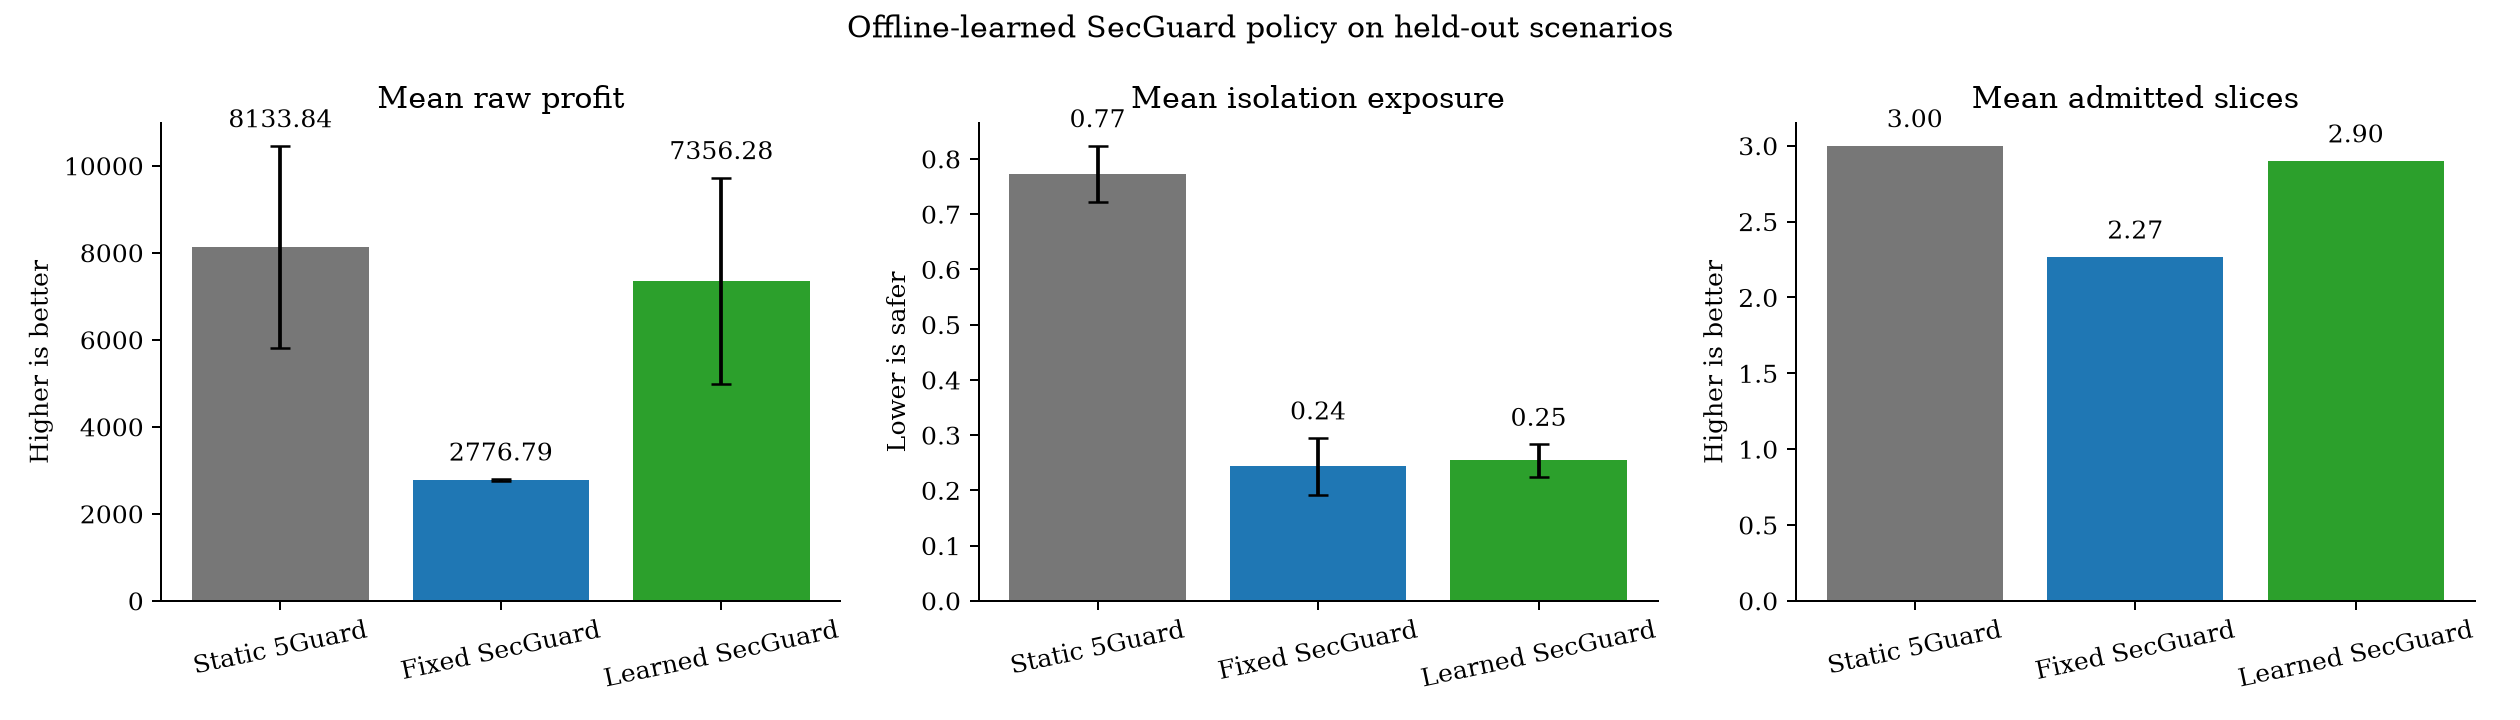
\includegraphics[width=0.96\textwidth]{learned_policy_comparison.png}
\caption{Static 5Guard, fixed SecGuard, and learned SecGuard on held-out
scenarios. Error bars show normal-approximation 95\% confidence intervals.}
\label{fig:comparison}
\end{figure*}

\subsection{Interpretation}
The fixed controller quarantines one request in every scenario and often spends
scarce resources on conservative upgrades. The learned controller raises the L1
and quarantine thresholds, allowing more low-risk traffic to remain shareable,
while lowering the L2 threshold to isolate moderate risks more decisively. Its
profit remains 9.56\% below static 5Guard, so the current contribution is not a
claim of free security. Instead, it recovers most economic performance while
retaining a large modeled security benefit.

\section{Threats to Validity and Required Extensions}
The present evidence is sufficient for proof of concept but not a final
deployment or journal claim.

\textbf{Data validity:} both training and test files come from the same dataset.
Random-Forest performance must be evaluated on another 5G testbed or with
leave-one-attack-family-out testing.

\textbf{Security construct validity:} Eq.~\eqref{eq:exposure} is a proxy. The
L1 sharing factor is assumed, and L2 is treated as eliminating cross-slice
exposure. A publishable extension should compute co-location from 5Guard's actual
node/link mappings and inject attack-induced resource pressure or QoS degradation.

\textbf{Allocation validity:} scenarios contain four requests and use IAR on the
synthetic topology. The full 5Guard ensemble, BRAIN topology, multiple loads,
arrival lengths, and at least 20--30 seeds per configuration are required.

\textbf{Statistical validity:} confidence intervals cover bootstrap scenarios,
not independent deployments. Multiple-comparison corrections and non-parametric
paired tests should accompany the final threshold sweep.

\textbf{Operational validity:} inference latency, monitoring-window size,
reconfiguration delay, migration downtime, and attacker adaptation are not yet
modeled. A false escalation can consume physical resources; a false negative can
leave co-tenants exposed.

The next evaluation should therefore add: (i) no-isolation and complete-isolation
baselines; (ii) logistic-regression, decision-tree, and oracle threshold
baselines; (iii) a Pareto frontier over profit and placement-derived exposure;
(iv) BRAIN and synthetic topologies at low, medium, and high load; (v) ablations
for SLA flooring, quarantine, and surrogate learning; and (vi) cross-dataset or
unseen-attack validation.

\section{Reproducibility}
The repository pins the upstream 5Guard revision and records every milestone,
artifact, limitation, and commit. Raw datasets and the upstream repository are
downloaded by scripts and excluded from version control. The experiment emits
machine-readable JSON, figures, feature importance, and confusion matrices.
Seventeen unit tests verify risk thresholds, SLA flooring, request non-mutation,
quarantine, exposure calculations, deterministic scenarios, and candidate
ordering. Numerical claims in this draft are sourced from
\texttt{artifacts/learned\_policy.json}.

\section{Conclusion}
SecGuard demonstrates that runtime 5G telemetry can be connected safely to
isolation-aware end-to-end slicing. Its first model estimates attack risk; its
adapter converts that risk to an SLA-safe 5Guard request; and its second ML stage
learns profit-aware thresholds under a security constraint. In preliminary
held-out scenarios, the learned policy substantially outperforms a conservative
fixed controller and retains most static 5Guard profit while reducing modeled
exposure. The result is a credible MTP proof of concept and a foundation for a
paper, but cross-dataset, placement-aware, full-ensemble, and large-topology
experiments remain necessary for publication-level evidence.

\balance
\bibliographystyle{IEEEtran}
\bibliography{references}
\end{document}

